\newcommand{\e} {\`e }
\newcommand{\E} {\`E }
\newcommand{\aee} {\'{e} }
\newcommand{\aea} {\`{a} }
\newcommand{\ai} {\`{\i} }
\newcommand{\ao} {\`{o} }
\newcommand{\au} {\`{u} }
\newcommand{\bit} {\begin{itemize} }
\newcommand{\eit} {\end{itemize} }



%\documentclass[handout]{beamer}
\documentclass{beamer}
\usepackage{pgfpages}
%\pgfpagesuselayout{2 on 1}[a4paper, border shrink=5mm]

\usepackage{helvet}
\renewcommand{\familydefault}{\sfdefault}

\usepackage{listings}
\usepackage{xcolor}
\usepackage{graphicx}
\usepackage{multicol}
\usepackage{caption}
\usepackage{makecell}
\usepackage{algpseudocode}  % sudo apt-get install texlive-science
\usepackage{algorithm}

\definecolor{UNIFIblue}{rgb}{0, 0.298, 0.494}  

\usecolortheme[named=UNIFIblue]{structure}

%\usetheme{PaloAlto}
\usetheme{Pittsburgh}
%\usetheme{Berkeley}


\definecolor{White}{rgb}{1.0,1.0,1.0}
\definecolor{Blue}{rgb}{0, 0.298, 0.494}
\definecolor{Pink}{rgb}{1.,0.75,0.8}
\definecolor{LRed}{rgb}{1.0,0.2,0.2}
\definecolor{Red}{rgb}{1.0,0.0,0.0}

\beamertemplatenavigationsymbolsempty

\setbeamertemplate{background}
{
\includegraphics[width=\paperwidth,height=\paperheight,keepaspectratio]{Immagine1}}

\begin{document}
\title{\textcolor{White}{Parallel Mean Shift Clustering}}  
\author{\textcolor{White}{Nicol\ao Pollini, Francesco Fantechi}}
\date{\textcolor{White}{22/06/2023}}
 

 
\frame{\titlepage} 

%%%%%%%%%%%%%%%%%%%%%%%%%%%%%%%%%%%%%%%%%%%%%%%%%%%%%%%%%%%%%%%%%%%%%%%%%

%%%%%%%%%%%%%%%%%%%%%%%%%%%%%%%%%%%%%%%%%%%%%%%%%%%%%%%%%%%%%%%%%%%%%%%%%
\setbeamertemplate{background}
{
\includegraphics[width=\paperwidth,height=\paperheight,keepaspectratio]{Immagine2}}





 
 
 \frame{\frametitle{Indice}
 \tableofcontents
 } 
 
 
 
 
 
 \setbeamercolor{date in head/foot}{fg=White, bg=UNIFIblue}
 \setbeamertemplate{footline}
 {
 	\begin{beamercolorbox}[ht=1ex,sep=1ex, center]{date in head/foot}
 		\insertshorttitle \ \ \hspace{2cm}  \insertsection  \ \ \ \insertsubsection \hfill\insertframenumber%/\inserttotalframenumber
 	\end{beamercolorbox}
 	
 }
 
 
 %%%%%%%%%%%%%%%%%%%%%%%%%%%%%%%%%%%%%%%%

\section{Obiettivo}
 
\frame{\frametitle{Obiettivo}
 	
	\bit
	\item {\color{Blue}Algoritmo MeanShift sequenziale}
	\item {\color{Blue} Parallelizzazione con OpenMP}
	\item {\color{Blue} Parallelizzazione con CUDA}
	\item {\color{Blue} Analisi e confronto dei risultati}
	\eit	
}

\section{Implementazione}
 
\frame{\frametitle{Implementazione}
 	
	\bit
	\item {\color{Blue} Segmentazione di immagini PPM a colori}
		\bit
			\item {\color{Blue} Spazio di clustering 5-dimensionale}
		\eit
	\item {\color{Blue} Linguaggio C++ per OpenMP e per CUDA}
	\item {\color{Blue} Codice versionato su GitHub:}
		\item[] {\color{Blue} \scriptsize - \url{https://github.com/francesco-ftk/Parallel-Mean-Shift-OpenMP}}
		\item[] {\color{Blue} \scriptsize - \url{https://github.com/francesco-ftk/Parallel-Mean-Shift-CUDA}}
	\item {\color{Blue} Test eseguiti su 3 macchine e 2 OS differenti}
	\eit	
}

\frame{\frametitle{Implementazione}

	\begin{center}
	\resizebox{0.9\textwidth}{!}{%
	\begin{tabular}{|c|c|c|c|c|}
	\hline
	\multicolumn{5}{|c|}{Machine 1}\\
	\hline
	\thead{OS} & \thead{CPU} & \thead{Number of Core \\ with Hyper-Threading} & \thead{RAM} & \thead{GPU}\\
	\hline
	\thead{Windows $ 10 $} & \thead{Intel(R) Core(TM) \\ i7-8750H} & \thead{$ 12 $} & \thead{$ 16 $ GB} & \thead{NVIDIA GeForce \\ GTX 1050 Ti}\\
	\hline
	\multicolumn{5}{|c|}{}\\
	\hline
	\multicolumn{5}{|c|}{Machine 2}\\
	\hline
	\thead{OS} & \thead{CPU} & \thead{Number of Core \\ with Hyper-Threading} & \thead{RAM} & \thead{GPU}\\
	\hline
	\thead{Ubuntu $ 20.04.5 $} & \thead{Intel(R) Core(TM) \\ i7-1165G7} & \thead{$ 8 $} & \thead{$ 16 $ GB} & \thead{NVIDIA GeForce \\ MX350}\\
	\hline
	\multicolumn{5}{|c|}{}\\
	\hline
	\multicolumn{5}{|c|}{Machine 3}\\
	\hline
	\thead{OS} & \thead{CPU} & \thead{Number of Core \\ with Hyper-Threading} & \thead{RAM} & \thead{GPU}\\
	\hline
	\thead{Windows $ 10 $} & \thead{Intel(R) Core(TM) \\ i7-7700K} & \thead{$ 8 $} & \thead{$ 32 $ GB} & \thead{NVIDIA GeForce \\ GTX 1080 Ti}\\
	\hline
	\end{tabular}}
	\end{center}
}


\section{Algoritmo MeanShift}
 
\frame{\frametitle{Algoritmo MeanShift}
 	
	\bit
	\item {\color{Blue} Clustering N-dimensionale}
	\item {\color{Blue} Applicazione del metodo di discesa del gradiente}
	\item {\color{Blue} Differenze con K-Means:}
		\bit
		\item {\color{Blue} no inizializzazione casuale,}
		\item {\color{Blue} rilevamento del numero di cluster,}
		\item {\color{Blue} parametri bandwidth e $\epsilon$,}
		\item {\color{Blue} complessità $O(n^{2})$}
		\eit
	\eit	
}
 
\frame{\frametitle{Algoritmo MeanShift}
 	
 	\begin{figure}
	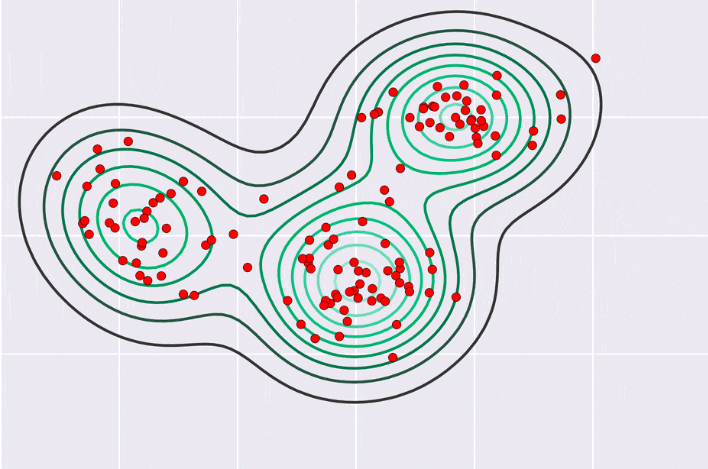
\includegraphics[width=0.6\textwidth]{Immagini/MeanShift0}
	\end{figure}
	\bit
	\item {\color{Blue} Inizializzazione dei centroidi}
	\item {\color{Blue} Filtraggio dei punti all'interno del supporto}
	\item {\color{Blue} Calcolo dello scostamento medio}
	\eit	
}
 
\frame{\frametitle{Algoritmo MeanShift}
 	
 	\begin{figure}
	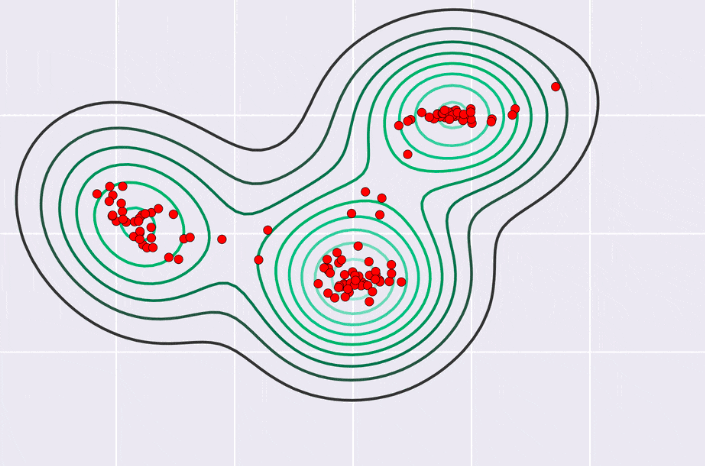
\includegraphics[width=0.6\textwidth]{Immagini/MeanShift1}
	\end{figure}
	\bit
	\item {\color{Blue} Aggiornamento dei centroidi}
	\item {\color{Blue} Confronto scostamento con $\epsilon$}
	\item[]
	\eit	
}
 
\frame{\frametitle{Algoritmo MeanShift}
 	
 	\begin{figure}
	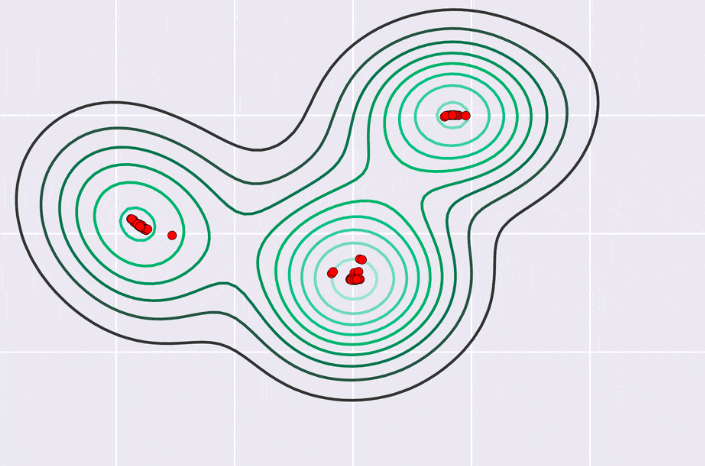
\includegraphics[width=0.6\textwidth]{Immagini/MeanShift2}
	\end{figure}
	\bit
	\item {\color{Blue} Iterazione se scostamento $> \epsilon$}
	\item[]
	\item[]
	\eit	
}
 
\frame{\frametitle{Algoritmo MeanShift}
 	
 	\begin{figure}
	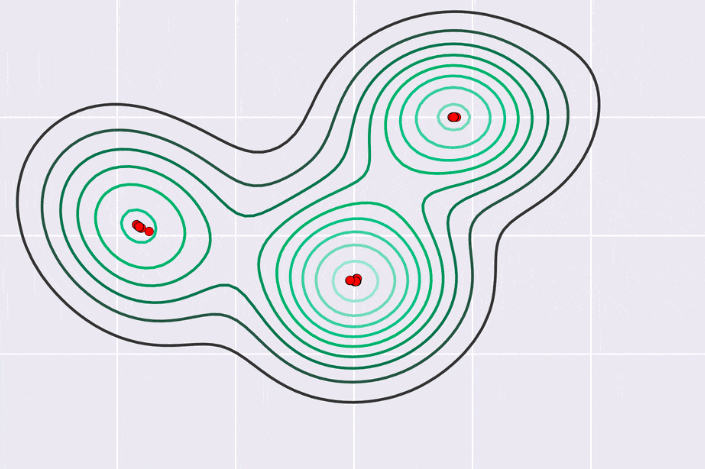
\includegraphics[width=0.6\textwidth]{Immagini/MeanShift3}
	\end{figure}
	\bit
	\item {\color{Blue} Termine iterazioni}
	\item {\color{Blue} Associazione delle mode}
	\item {\color{Blue} Raggruppamento in cluster}
	\eit	
}

\subsection{Versione sequenziale}
 
\frame{\frametitle{Versione sequenziale}
 	
	\bit
	\item {\color{Blue} AoS:}
		\bit
			\item {\color{Blue} punti collocati sequenzialmente in un unico vettore,}
			\item {\color{Blue} punti rappresentati da una Struct di 5 campi}
			\item {\color{Blue} dati localmente vicini, accesso più semplice.}
		\eit
	\item {\color{Blue} SoA:}
		\bit
		\item {\color{Blue} punti distribuiti su 5 array,}
		\item {\color{Blue} struttura più complessa, ma meglio allineabile alla cache,}
		\item {\color{Blue} accesso coalesced, vantaggi su versioni parallelizzate}
		\eit
	\eit	
	\begin{figure}
	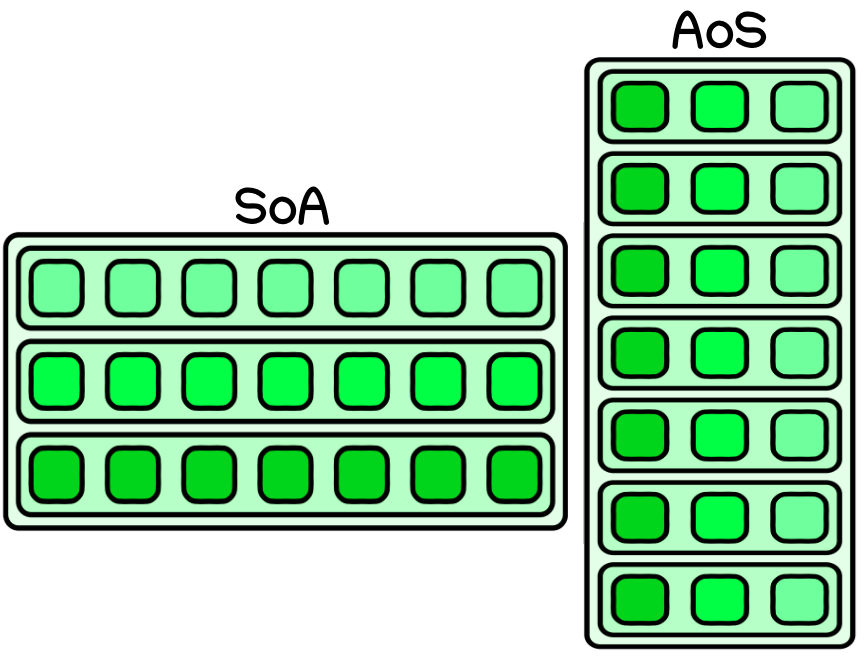
\includegraphics[width=0.4\textwidth]{Immagini/SoAvsAoS}
	\end{figure}
}

\section{Parallelizzazione}
 
\frame{\frametitle{Parallelizzazione}
 	
	\bit
	\item {\color{Blue} Calcolo delle mode:}
		\bit
			\item {\color{Blue} imbarazzantemente parallela,}
			\item {\color{Blue} complessità $O(n^{2})$}
			\item[] {\color{Blue} $\rightarrow$ parallelizzato}
		\eit
	\item {\color{Blue} Raggruppamento in cluster:}
		\bit
		\item {\color{Blue} richiede collaborazione,}
		\item {\color{Blue} complessità O(n)}
		\item[] {\color{Blue} $\rightarrow$ non parallelizzato}
		\eit
	\eit	
}

\subsection{OpenMP}

\frame{\frametitle{OpenMP}

	\bit
	\item {\color{Blue} Framework per parallelizzazione in modalità implicit threading}
	\item {\color{Blue} Creazione di thread e parallelizzazione con direttive pragma}
	\item {\color{Blue} Divisione del carico di lavoro con paradigma fork-join}
	\eit
	\begin{figure}
	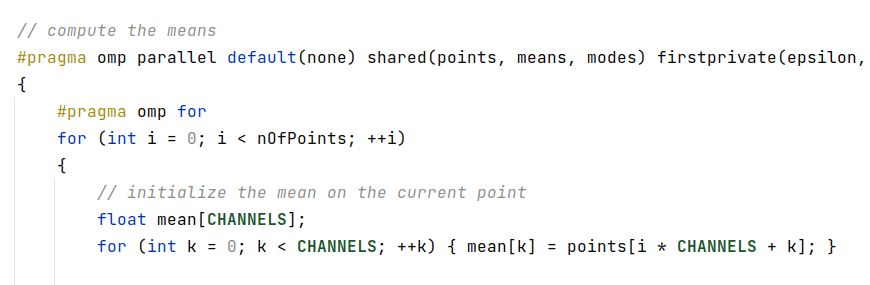
\includegraphics[width=0.9\textwidth]{Immagini/Code_OpenMP_1}
	\end{figure}
}
 
\frame{\frametitle{OpenMP}
 	
	\bit
	\item {\color{Blue} Divisione equa dei punti da processare}
	\item {\color{Blue} Calcolo della mode in modo indipendente:}
		\bit
		\item {\color{Blue} nessuna necessità di comunicazione}
		\eit
	\item {\color{Blue} Riduzione effettuata in modo sequenziale}
	\item {\color{Blue} Test effettuati sia con AoS che SoA}
	\eit	
}

\frame{\frametitle{OpenMP}

	\begin{figure}
	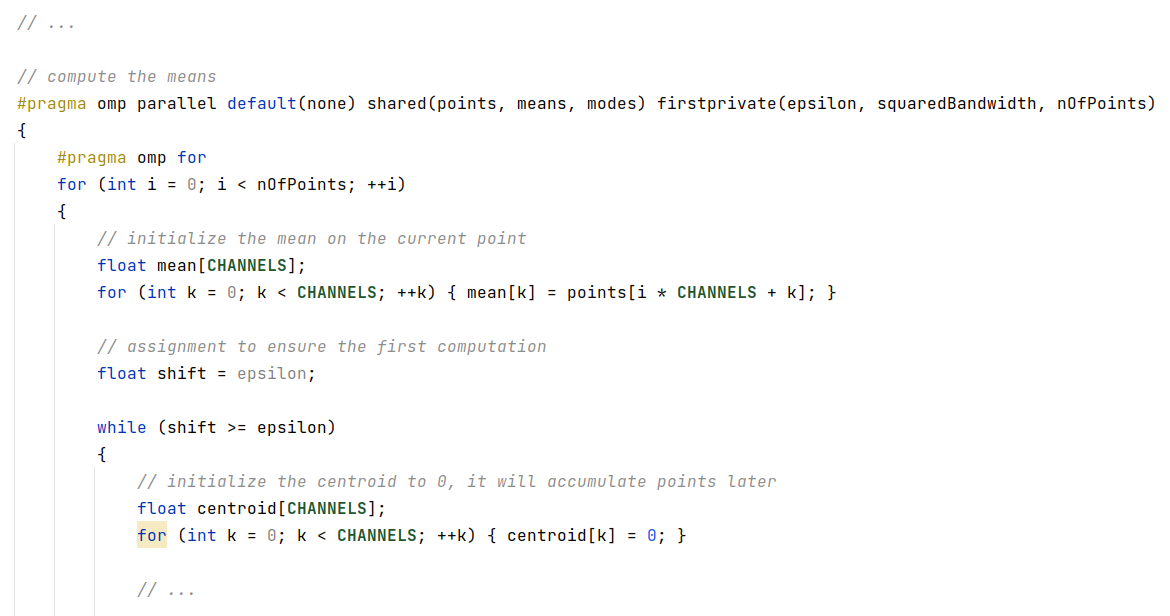
\includegraphics[width=\textwidth]{Immagini/Code_OpenMP}
	\end{figure}
}

\subsection{CUDA}
 
\frame{\frametitle{CUDA}

	\bit
	\item {\color{Blue} Architettura per parallelizzazione su GPU Nvidia}
	\item {\color{Blue} GPU (device) vista come coprocessore della CPU (host)}
	\item {\color{Blue} Alto numero di unità di calcolo}
	\item {\color{Blue} Varie strutture di memoria}
	\eit
	\begin{figure}
	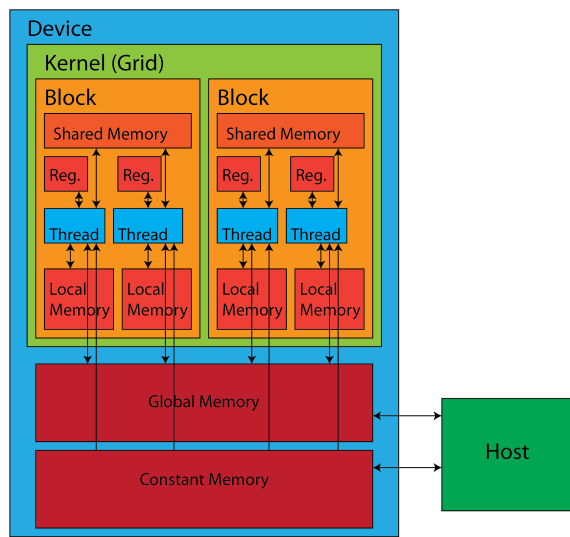
\includegraphics[width=0.5\textwidth]{Immagini/Memory}
	\end{figure}
}
 
\frame{\frametitle{CUDA}
 	
	\bit
	\item {\color{Blue} Ogni Thread è responsabile del calcolo di una singola mode}
	\item {\color{Blue} I Block di thread rappresentano chunk 2D dell'immagine}
	\item {\color{Blue} Ogni punto viene letto da tutti i thread per ogni iterazione:}
		\bit
		\item {\color{Blue} condivisione dei dati a livello di blocco,}
		\item {\color{Blue} strategia di Tiling per sfruttare la Shared Memory}
		\eit
	\item {\color{Blue} Riduzione effettuata all'esterno del kernel}
	\eit	
	\begin{figure}
	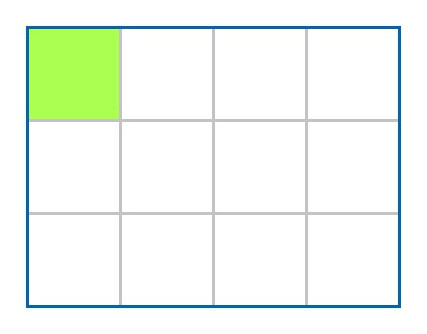
\includegraphics[width=0.3\textwidth]{Immagini/Tiling0}
	\end{figure}
}
 
\frame{\frametitle{CUDA}

	\begin{figure}
	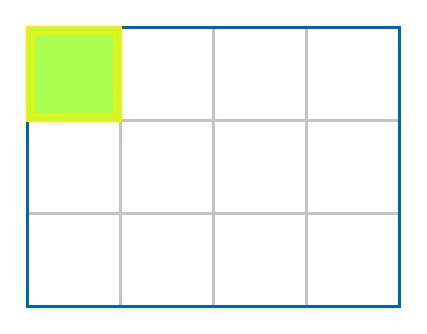
\includegraphics[width=0.7\textwidth]{Immagini/Tiling1}
	\end{figure}
}
 
\frame{\frametitle{CUDA}

	\begin{figure}
	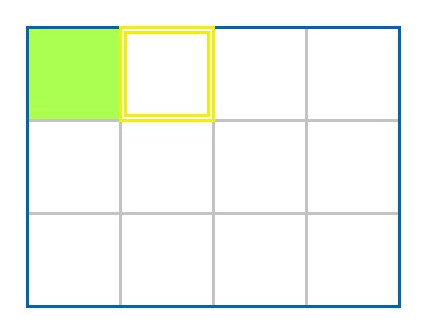
\includegraphics[width=0.7\textwidth]{Immagini/Tiling2}
	\end{figure}
}
 
\frame{\frametitle{CUDA}

	\begin{figure}
	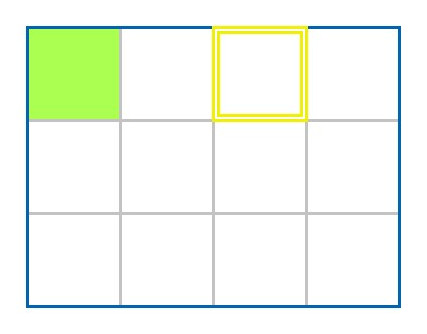
\includegraphics[width=0.7\textwidth]{Immagini/Tiling3}
	\end{figure}
}
 
\frame{\frametitle{CUDA}

	\begin{figure}
	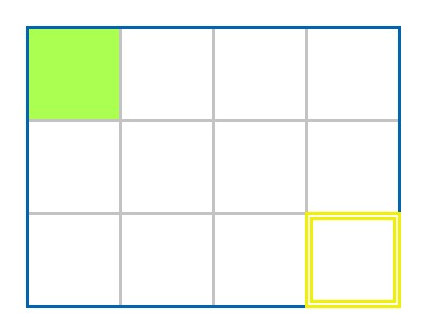
\includegraphics[width=0.7\textwidth]{Immagini/Tiling4}
	\end{figure}
}
 
\frame{\frametitle{CUDA}

	\begin{figure}
	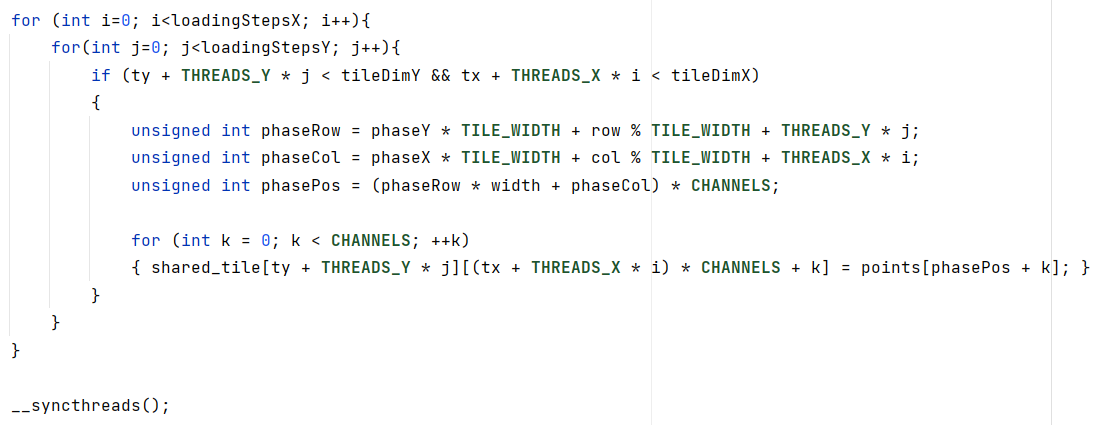
\includegraphics[width=\textwidth]{Immagini/shared-load}
	\end{figure}
}

\frame{\frametitle{CUDA}

	\begin{figure}
	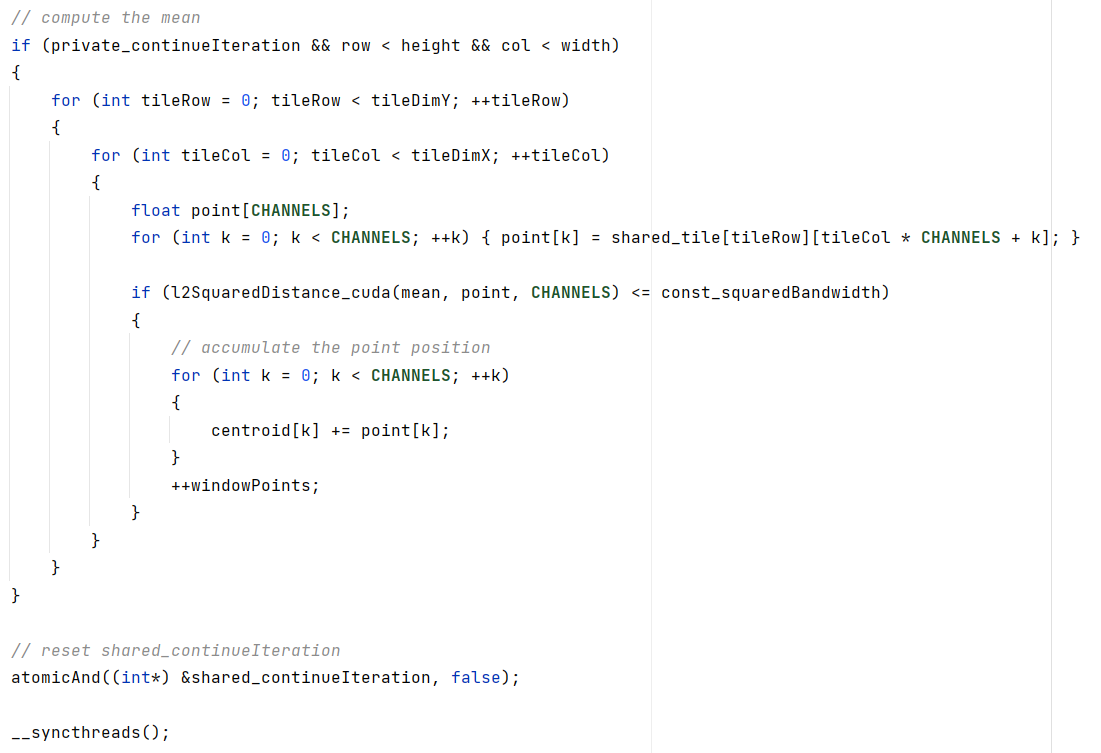
\includegraphics[width=\textwidth]{Immagini/shared-consume}
	\end{figure}
}
 
\frame{\frametitle{CUDA}
 	
	\bit
	\item {\color{Blue} Il numero di iterazioni per punto è stocastico:}
		\bit
		\item {\color{Blue} alcuni thread potrebbero terminare prematuramente,}
		\item {\color{Blue} il tiling necessita che tutti i thread carichino i dati}
		\eit
	\item {\color{Blue} Introduzione di una comunicazione a livello di blocco:}
		\bit
		\item {\color{Blue} una variabile condivisa coordina il numero di iterazioni,}
		\item {\color{Blue} una variabile privata stabilisce se consumare o meno i dati}
		\eit
	\eit	
	
	\begin{figure}
	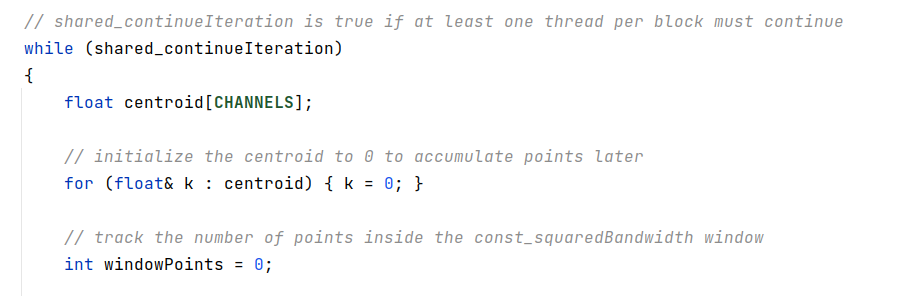
\includegraphics[width=0.9\textwidth]{Immagini/shared-variable}
	\end{figure}
}
 
\frame{\frametitle{CUDA}

	\begin{figure}
	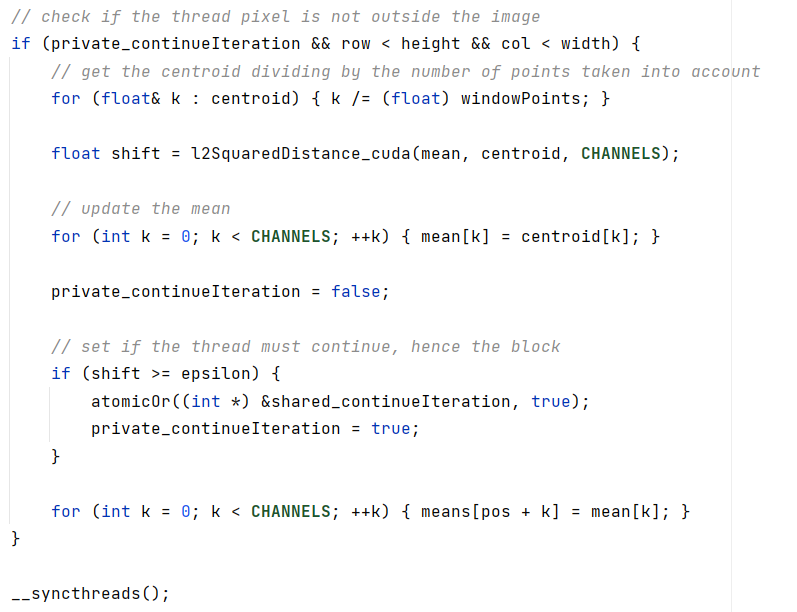
\includegraphics[width=0.9\textwidth]{Immagini/iteration-end}
	\end{figure}
}


\section{Risultati}
 
\frame{\frametitle{Risultati}

	\bit
	\item {\color{Blue} Clustering apprezzabile}
	\item {\color{Blue} Stesso risultato finale con entrambi i metodi}
		\bit
		\item {\color{Blue} $\rightarrow$ Ripetibilità}
		\eit
	\item[] {\begin{figure}
	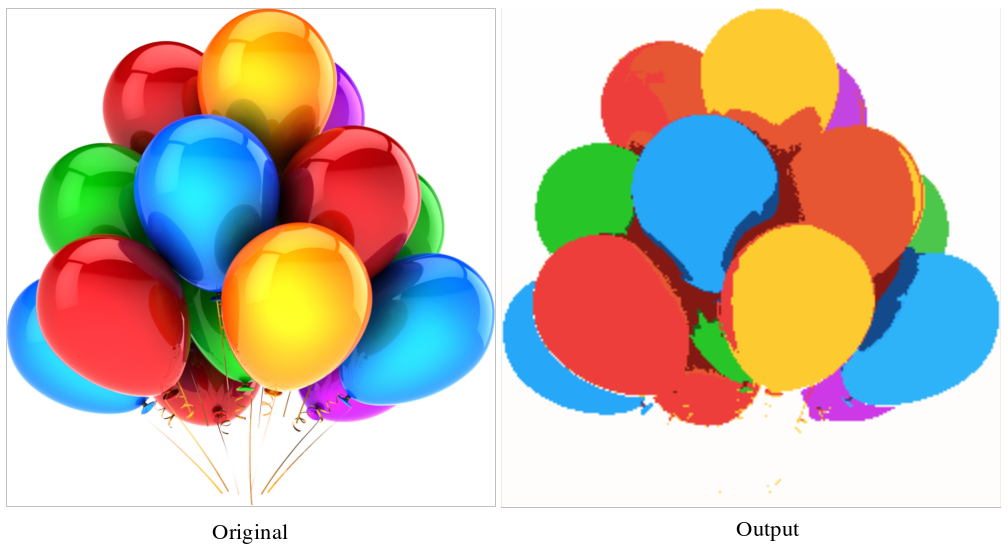
\includegraphics[width=0.5\textwidth]{Immagini/Output}
	\end{figure}}
	\item {\color{Blue} Performance nettamente differenti}
	\eit
}
 
\frame{\frametitle{Risultati}

	\begin{center}
	\resizebox{\textwidth}{!}{%
	\begin{tabular}{|c|c|c|c|c|c|}
	\hline
	\multicolumn{6}{|c|}{Machine 1}\\
	\hline
	\thead{Image dimension} & \thead{Sequential AoS} & \thead{Sequential SoA} & \thead{OpenMP AoS} & \thead{OpenMP SoA} & \thead{CUDA}\\
	\hline
	\thead{$ 100\times100$ pixel} & \thead{$ 102810ms$} & \thead{$ 102188ms $} & \thead{$  17047ms $}  & \thead{$  15657ms $} & \thead{$  10477ms $}\\
	\hline
	\thead{$ 250\times250$ pixel} & \thead{$ 3955082ms $} & \thead{$ 3886222ms $} & \thead{$ 575754ms $}  & \thead{$ 554569ms $} & \thead{$ 276233ms $}\\
	\hline
	\multicolumn{6}{|c|}{}\\
	\hline
	\multicolumn{6}{|c|}{Machine 2}\\
	\hline
	\thead{Image dimension} & \thead{Sequential AoS} & \thead{Sequential SoA} & \thead{OpenMP AoS} & \thead{OpenMP SoA} & \thead{CUDA}\\
	\hline
	\thead{$ 100\times100$ pixel} & \thead{$ 37370ms $} & \thead{$ 35758ms $} & \thead{$ 9937ms $}  & \thead{$ 10056ms $} & \thead{$ 12892ms $}\\
	\hline
	\thead{$ 250\times250$ pixel} & \thead{$ 1442048ms $} & \thead{$ 1393829ms $} & \thead{$ 467553ms $}  & \thead{$ 494691ms $} & \thead{$ 355589ms $}\\
	\hline
	\multicolumn{6}{|c|}{}\\
	\hline
	\multicolumn{6}{|c|}{Machine 3}\\
	\hline
	\thead{Image dimension} & \thead{Sequential AoS} & \thead{Sequential SoA} & \thead{OpenMP AoS} & \thead{OpenMP SoA} & \thead{CUDA}\\
	\hline
	\thead{$ 100\times100$ pixel} & \thead{$ 87317ms $} & \thead{$ 86241ms $} & \thead{$ 16547ms $}  & \thead{$ 15367ms $} & \thead{$ 3009ms $}\\
	\hline
	\thead{$ 250\times250$ pixel} & \thead{$ 3339803ms $} & \thead{$ 3309131ms $} & \thead{$ 601750ms $}  & \thead{$ 574439ms $} & \thead{$ 56213ms  $}\\
	\hline
	\end{tabular}}
	\end{center}
}
 
\frame{\frametitle{Risultati}
	
	\begin{figure}
	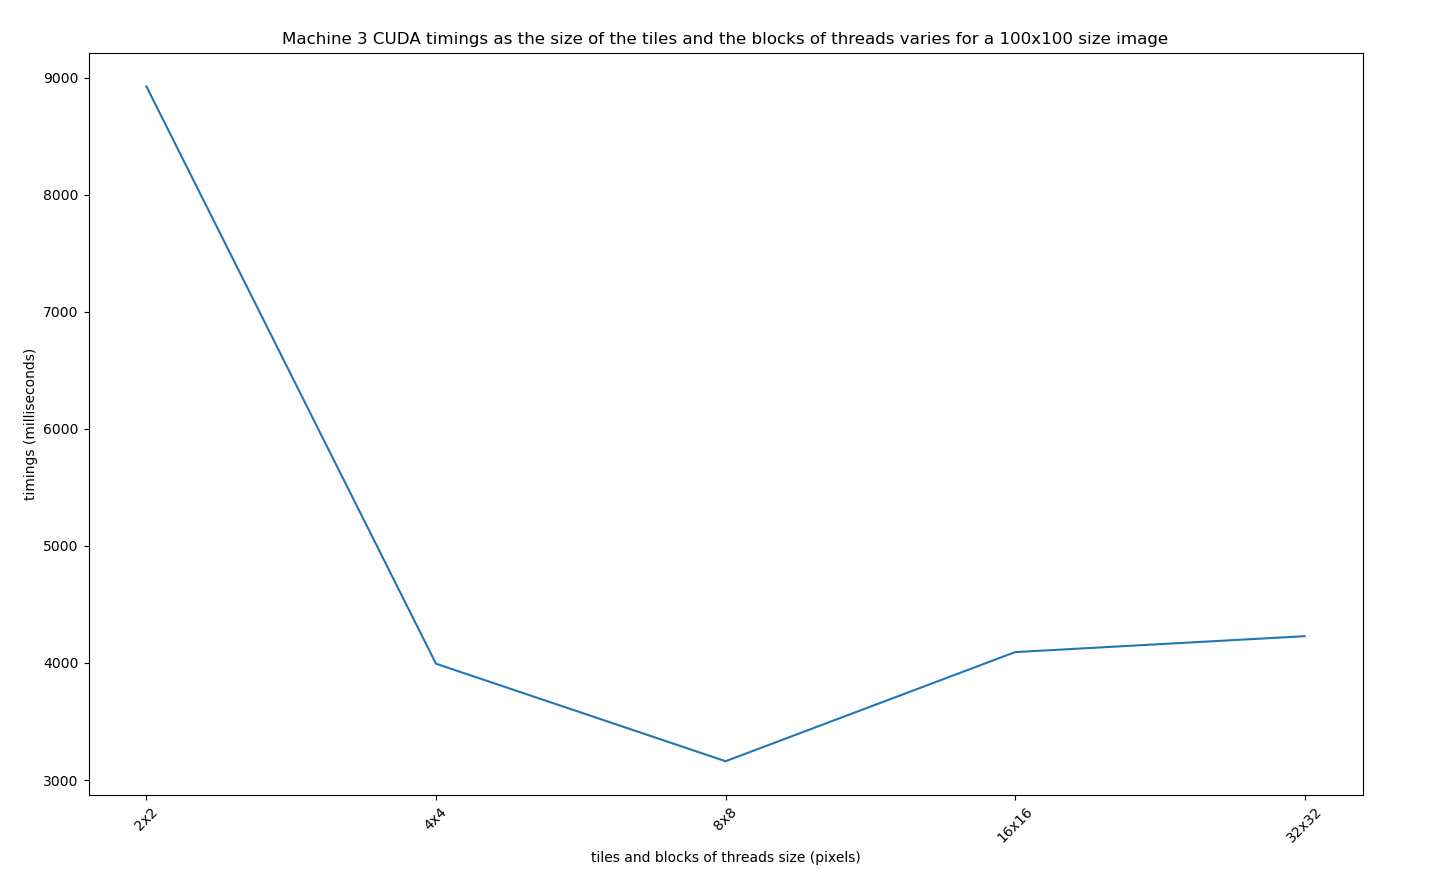
\includegraphics[width=\textwidth]{Immagini/Timings_Varying_Tiles}
	\end{figure}
}

\frame{\frametitle{Risultati}

	\begin{center}
	\resizebox{0.7\textwidth}{!}{%
	\begin{tabular}{|c|c|c|c|}
	\hline
	\multicolumn{4}{|c|}{Machine 1}\\
	\hline
	\thead{Image dimension} & \thead{OpenMP AoS} & \thead{OpenMP SoA} & \thead{CUDA}\\
	\hline
	\thead{$ 100\times100$ pixel} & \thead{$ 6.0 $}  & \thead{$ 6.5 $} & \thead{$ 9.8 $}\\
	\hline
	\thead{$ 250\times250$ pixel} & \thead{$ 6.9 $}  & \thead{$ 7.0 $} & \thead{$ 14 $}\\
	\hline
	\multicolumn{4}{|c|}{}\\
	\hline
	\multicolumn{4}{|c|}{Machine 2}\\
	\hline
	\thead{Image dimension} & \thead{OpenMP AoS} & \thead{OpenMP SoA} & \thead{CUDA}\\
	\hline
	\thead{$ 100\times100$ pixel} & \thead{$ 3.7 $}  & \thead{$ 3.6 $} & \thead{$ 2.9 $}\\
	\hline
	\thead{$ 250\times250$ pixel} & \thead{$ 3.0 $}  & \thead{$ 2.8 $} & \thead{$ 4.1 $}\\
	\hline
	\multicolumn{4}{|c|}{}\\
	\hline
	\multicolumn{4}{|c|}{Machine 3}\\
	\hline
	\thead{Image dimension} & \thead{OpenMP AoS} & \thead{OpenMP SoA} & \thead{CUDA}\\
	\hline
	\thead{$ 100\times100$ pixel} & \thead{$ 5.3 $}  & \thead{$ 5.6 $} & \thead{$ 29.0 $}\\
	\hline
	\thead{$ 250\times250$ pixel} & \thead{$ 5.6 $}  & \thead{$ 5.8 $} & \thead{$ 59.4 $}\\
	\hline
	\end{tabular}}
	\end{center}
}

\frame{\frametitle{Risultati}

	\begin{figure}
	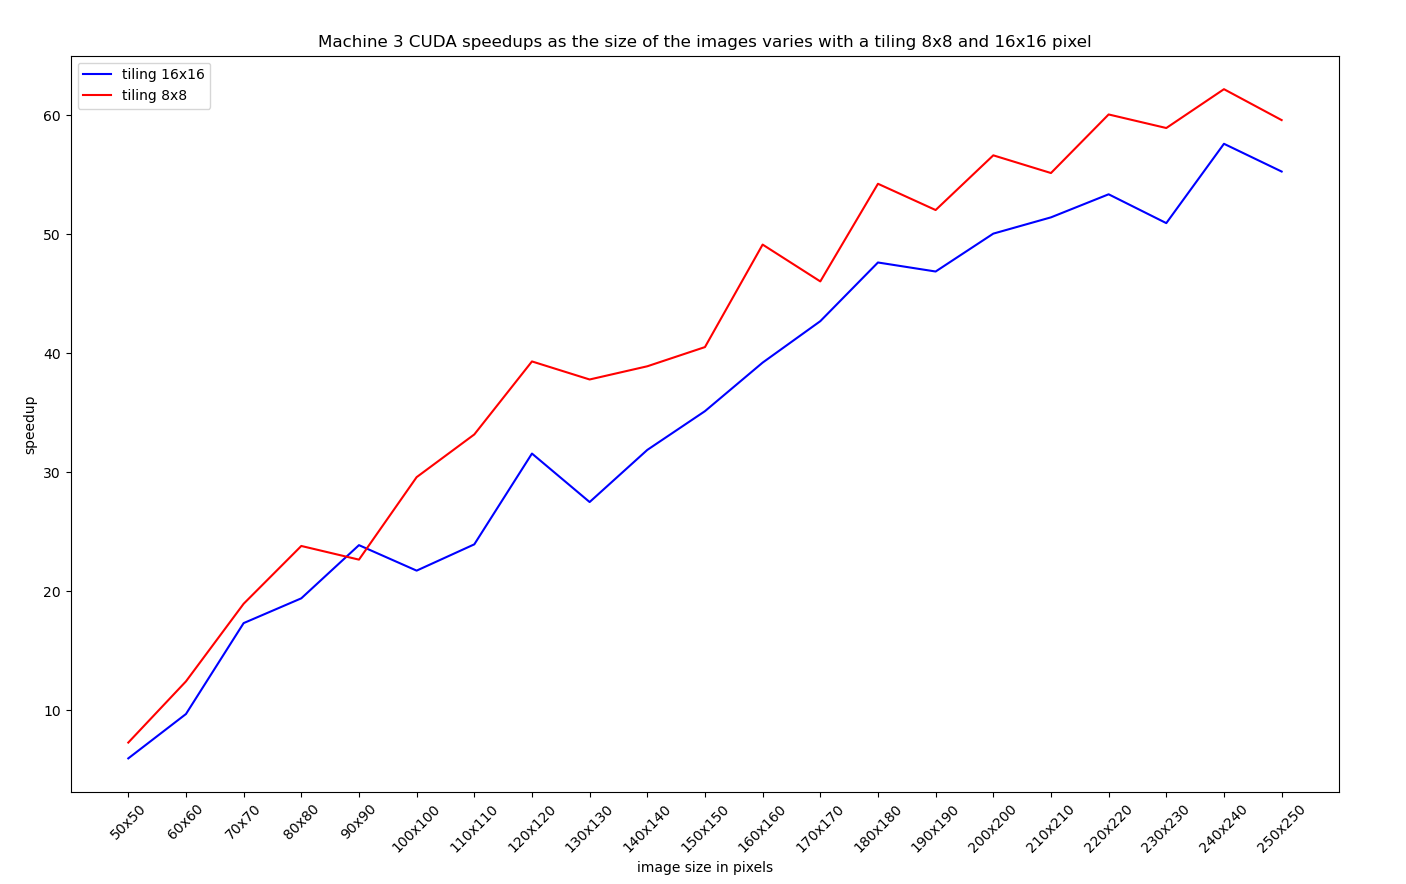
\includegraphics[width=\textwidth]{Immagini/Speedups_Varying_Size}
	\end{figure}
}


\section{Conclusioni}
 
\frame{\frametitle{Conclusioni}

	\bit
	\item {\color{Blue} OpenMP:}
		\bit
		\item {\color{Blue} struttura SoA vantaggiosa in alcune circostanze,}
		\item {\color{Blue} parallelizzazione efficace con speedup sublineare}
		\eit
	\item {\color{Blue} CUDA:}
		\bit
		\item {\color{Blue} risultati significativamente migliori,}
		\item {\color{Blue} speedup in crescita con l'aumento della dimensione del problema,}
		\item {\color{Blue} strategie come tiling e uso della shared memory sono risultate molto efficaci}
		\eit
	\eit
}

\end{document}
